\section{Harder multi-\textsc{mnist} Experiment}
\label{app:mnist_inout}
We created a version of the multi-\textsc{mnist} dataset, where objects can appear or disappear at an arbitrary point in time.
It differs from the dataset described in \Cref{sec:expr_mnist}, where all digits are present throughout the sequence.
All other dataset parameters are the same as in \Cref{sec:expr_mnist}.
\Cref{fig:mnist_rec_in_and_out} shows an example sequence and \textsc{mlp}-\gls{SQAIR} reconstructions with marked glimpse locations.
The model has no trouble detecting new digits in the middle of the sequence and rediscovering a digit that was previously present.

\begin{figure}
    \centering
    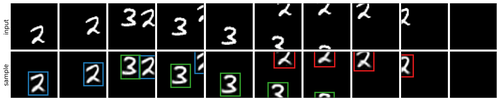
\includegraphics[width=\linewidth]{figures/SQAIR/mnist_rec/in_and_out.png}
    \caption{\gls{SQAIR} trained on a harder version of moving-\textsc{mnist}. Input images (top) and \gls{SQAIR} reconstructions with marked glimpse locations (bottom)}
    \label{fig:mnist_rec_in_and_out}
\end{figure}